\def\mytitle{IMPLEMENTATION OF BOOLEAN LOGIC IN AVRGCC}
\def\myauthor{B JAYASRI}
\def\contact{r180747@rguktrkv.ac.in}
\def\mymodule{Future Wireless Communications (FWC)}
\documentclass[journal,12pt,twocolumn]{IEEEtran}

\usepackage{setspace}
\usepackage{gensymb}
\usepackage{xcolor}
\usepackage{caption}
\usepackage[hyphens,spaces,obeyspaces]{url}
\usepackage[cmex10]{amsmath}
\usepackage{mathtools}
\singlespacing
\usepackage{amsthm}
\usepackage{mathrsfs}
\usepackage{txfonts}
\usepackage{stfloats}
\usepackage{cite}
\usepackage{cases}
\usepackage{subfig}
\usepackage{longtable}
\usepackage{multirow}
\twocolumn


\usepackage{graphicx}
\graphicspath{{./images/}}
\usepackage[colorlinks,linkcolor={black},citecolor={blue!80!black},urlcolor={blue!80!black}]{hyperref}
\usepackage[parfill]{parskip}
\usepackage{lmodern}
\usepackage{tikz}
\usepackage{circuitikz}
\usepackage{karnaugh-map}
\usepackage{pgf}
\usepackage[hyphenbreaks]{breakurl}

\usepackage{tabularx}
\usetikzlibrary{calc}

\renewcommand*\familydefault{\sfdefault}
\usepackage{watermark}
\usepackage{lipsum}
\usepackage{xcolor}
\usepackage{listings}
\usepackage{float}
\usepackage{titlesec}
\usepackage{enumitem}
\DeclareMathOperator*{\Res}{Res}
\renewcommand\thesection{\arabic{section}}
\renewcommand\thesubsection{\thesection.\arabic{subsection}}
\renewcommand\thesubsubsection{\thesubsection.\arabic{subsubsection}}

\renewcommand\thesectiondis{\arabic{section}}
\renewcommand\thesubsectiondis{\thesectiondis.\arabic{subsection}}
\renewcommand\thesubsubsectiondis{\thesubsectiondis.\arabic{subsubsection}}
\titlespacing{\subsection}{1pt}{\parskip}{3pt}
\titlespacing{\subsubsection}{0pt}{\parskip}{-\parskip}
\titlespacing{\paragraph}{0pt}{\parskip}{\parskip}
\newcommand{\figuremacro}[5]{
    \begin{figure}[#1]
        \centering
        \includegraphics[width=#5\columnwidth]{#2}
        \caption[#3]{\textbf{#3}#4}
        \label{fig:#2}
    \end{figure}
}

\lstset{
frame=single, 
breaklines=true,
columns=fullflexible
}
\title{\mytitle}
\author{\myauthor\hspace{1em}\\\contact\\IITH\hspace{0.5em}-\hspace{0.6em}\mymodule}
\date{20-12-2022}
\def\inputGnumericTable{}                                 %%
\lstset{
frame=single, 
breaklines =true,
columns= fullflexible
}
 \begin{document}
\theoremstyle{definition}
\newtheorem{theorem}{Theorem}[section]
\newtheorem{problem}{Problem}
\newtheorem{proposition}{Proposition}[section]
\newtheorem{lemma}{Lemma}[section]
\newtheorem{corollary}[theorem]{Corollary}
\newtheorem{example}{Example}[section]
\newtheorem{definition}{Definition}[section]
%\newtheorem{algorithm}{Algorithm}[section]
%\newtheorem{cor}{Corollary}
\newcommand{\BEQA}{\begin{eqnarray}}
\newcommand{\EEQA}{\end{eqnarray}}
\newcommand{\define}{\stackrel{\triangle}{=}}
%\bibliographystyle{IEEEtran}

\vspace{3cm}
\maketitle
\tableofcontents
  \section{\textbf{Question}}
  \begin{enumerate}     
\item  For the 3-bit binary counter shown in the figure, the output increments at every positive 
transition in the clock (CLK). Assume ideal diodes and the starting state of the counter as 
000. If output high is 1 V and output low is 0 V, the current I (in mA) flowing through the 
50 Ω resistor during the 5th clock cycle is (up to one decimal place)
\begin{figure}[H]
\centering
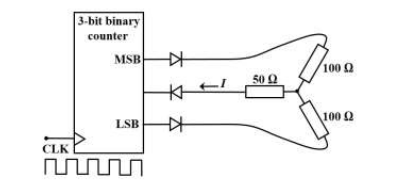
\includegraphics[width=\columnwidth]{figs/circuit.png}
\caption{circuit}
\label{fig:lcd}
\end{figure}
\end{enumerate}
\section{\textbf{Components}}
\begin{tabularx}{0.46\textwidth} { 
  | >{\centering\arraybackslash}X 
  | >{\centering\arraybackslash}X 
  | >{\centering\arraybackslash}X
  | >{\centering\arraybackslash}X | }
\hline
\textbf{Component}& \textbf{Values} & \textbf{Quantity}\\
\hline
Arduino & UNO & 1 \\  
\hline
JumperWires & M-M & 15 \\ 
\hline
LCD & &1\\
\hline
Bread board & & 1\\
\hline
     \end{tabularx}
\section{\textbf{LCD PINS}}
 \begin{figure}[H]
\centering
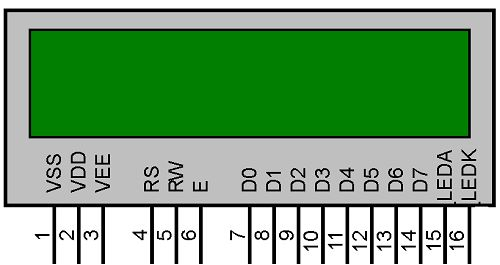
\includegraphics[width=\columnwidth]{figs/LCD.jpg}
\caption{LCD}
\label{fig:lcd}
\end{figure} 
\section{\textbf{Implementation}}
  \begin{tabularx}{0.46\textwidth} { 
  | >{\centering\arraybackslash}X 
  | >{\centering\arraybackslash}X  | }
\hline
\textbf{Arduino PIN} & \textbf{LCD} \\ 
\hline
D7 & RS\\
\hline
D8 & EN\\
\hline
D9 & 11\\
\hline
D10 & 12\\
\hline
D11 & 13\\
\hline
D12 & 14\\
\hline
5V & VCC\\
\hline
\end{tabularx}
\begin{center}
    Connections
\end{center}
\section{\textbf{Procedure}}
    1. Connect the circuit as per the above table.\\
    2. connect the LCD to Arduino UNO\\
\\ \begin{tabularx}{0.5\textwidth} { 
  | >{\centering\arraybackslash}X |}
  \hline
https://github.com/r180747/FWC-1/blob/main/AVR-GCC/code.c
  \hline
  \end{tabularx}
    \section{\textbf{LCD OUTPUT}}
 \begin{figure}[H]
\centering
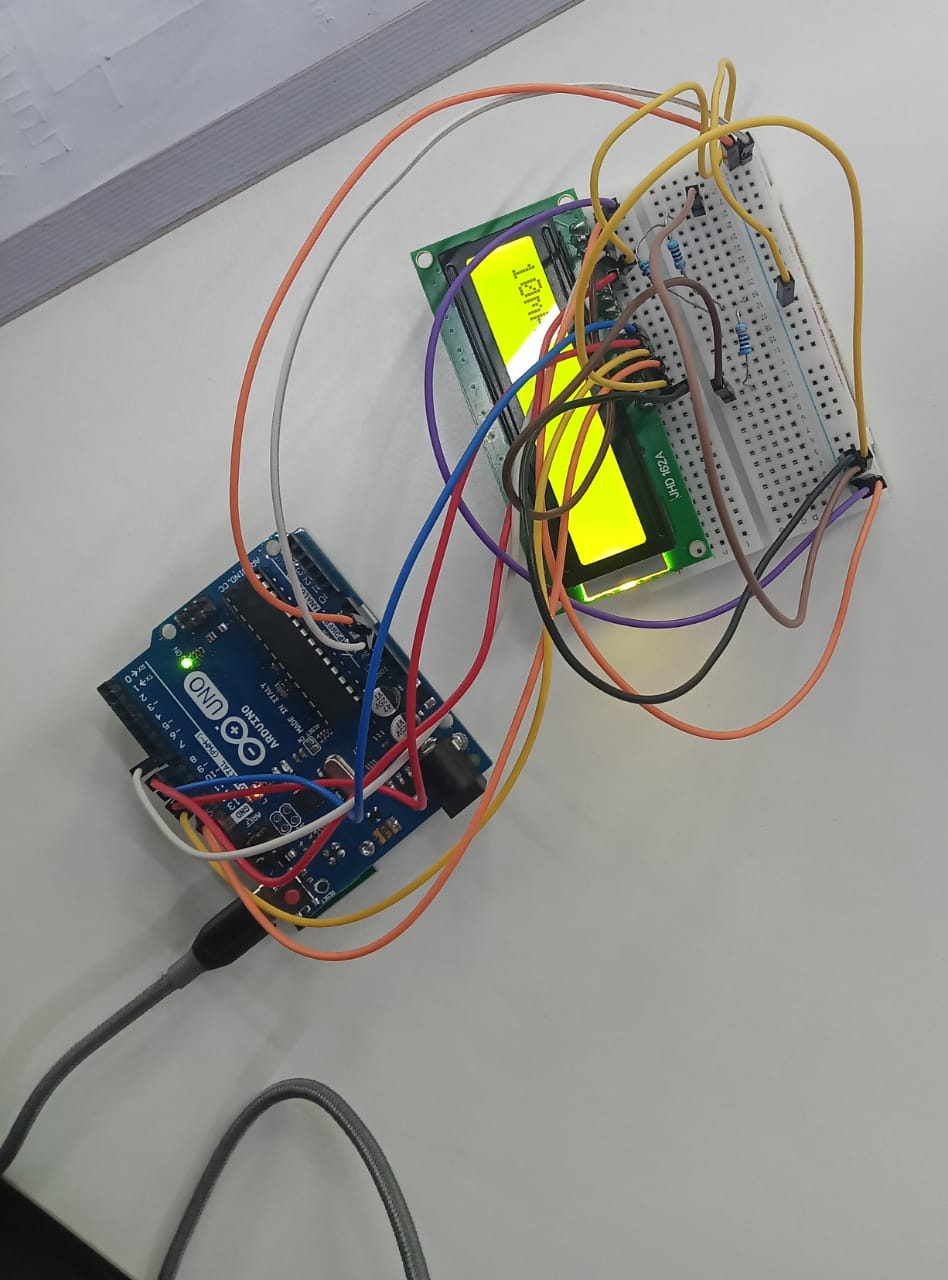
\includegraphics[width=\columnwidth]{figs/figavr.jpeg}
\caption{output}
\label{fig:figavr}
\end{figure}


 \bibliographystyle{ieeetr}
\end{document}
